\section{Avaliação de desempenho e funcionalidade}
Nessa sessão será apresentado os ambientes dos cenários de testes, principalmente como foram configurados e seus respectivos \textit{hardwares}. Também será exposto os resultados dos experimentos realizados neste trabalho.
\subsection{Equipamentos}

Como explicado na seção \ref{Metodologia}, o testes serão realizados seguindo cenários com diversos equipamentos, que devem realizar funções diferentes dependendo do cenário selecionado.
A coleta de métricas de consumo de processador, memória, entrada e saída de \textit{bits} pela interface de rede
foram realizadas usando o \textit{software} Prometheus em conjunto com o Grafana para a visualização gráfica dos dados.

\begin{table}[H]
\centering
\label{tab:freq-conf}
\begin{tabular}{cc|}
\hline
\rowcolor[HTML]{DFDFDF} 
\multicolumn{2}{|c|}{\cellcolor[HTML]{DFDFDF}A - Thinkpad T440s}               \\ \hline
\rowcolor[HTML]{EFEFEF} 
\multicolumn{1}{|c|}{\cellcolor[HTML]{EFEFEF}Processador}         & Intel\textregistered\space Core\texttrademark\space i5 4200U          \\ \hline
\multicolumn{1}{|c|}{RAM}                    & 8GB DDR3               \\ \hline
\rowcolor[HTML]{EFEFEF} 
\multicolumn{1}{|c|}{\cellcolor[HTML]{EFEFEF}SO} & NixOS GNU/Linux                   \\ \hline
\multicolumn{1}{|c|}{\textit{kernel}}                   & 6.1.79          \\ \hline \hline
\rowcolor[HTML]{DFDFDF} 
\multicolumn{2}{|c|}{\cellcolor[HTML]{DFDFDF}B - Raspberry Pi 4}                 \\ \hline
\rowcolor[HTML]{EFEFEF} 
\multicolumn{1}{|c|}{\cellcolor[HTML]{EFEFEF}Processador} & Broadcom BCM2711 \\ \hline
\multicolumn{1}{|c|}{RAM} & 4GB LPDDR4  \\ \hline
\rowcolor[HTML]{EFEFEF} 
\multicolumn{1}{|c|}{\cellcolor[HTML]{EFEFEF}SO}                 & RPiOS Lite GNU/Linux     \\ \hline
\multicolumn{1}{|c|}{\textit{kernel}}   & 6.6.20+rpt-rpi-v8    \\ \hline 
\end{tabular}
\begin{tabular}[h]{cc|} \hline
\rowcolor[HTML]{DFDFDF} 
\multicolumn{2}{|c|}{\cellcolor[HTML]{DFDFDF}C - \textit{Custom Build}}              \\ \hline
\rowcolor[HTML]{EFEFEF} 
\multicolumn{1}{|c|}{\cellcolor[HTML]{EFEFEF}Processador} & Intel\textregistered\space Xeon\textregistered\space E5-2670v3            \\ \hline
\multicolumn{1}{|c|}{RAM}                         & 16GB DDR4 ECC              \\ \hline
\rowcolor[HTML]{EFEFEF} 
\multicolumn{1}{|c|}{\cellcolor[HTML]{EFEFEF}SO}         & NixOS GNU/Linux \\ \hline
\multicolumn{1}{|c|}{\textit{kernel}}           & 6.1.79  \\ \hline \hline
\rowcolor[HTML]{DFDFDF} 
\multicolumn{2}{|c|}{\cellcolor[HTML]{DFDFDF}D - TPLink WR741ND}                 \\ \hline
\rowcolor[HTML]{EFEFEF} 
\multicolumn{1}{|c|}{\cellcolor[HTML]{EFEFEF}Banda} & \textit{FastEthernet} 100Mbit/s         \\ \hline
\multicolumn{1}{|c|}{\textit{Firmware}}                        & OpenWRT                \\ \hline
\rowcolor[HTML]{EFEFEF} 
\multicolumn{1}{|c|}{\cellcolor[HTML]{EFEFEF}Núm. Portas}         & 4        \\ \hline
\multicolumn{1}{|c|}{Lançamento}           & 2016    \\ \hline
\end{tabular}
\caption{Especificação dos Equipamentos}
\end{table}
%Para a realização dos cenários de testes foram criados \textit{testbeds} compostos por três computadores, um roteador e um \textit{switch}. 
%\subsection{\textit{Testbed}}
%Para a realização dos dois cenários de testes foi criado uma \textit{Testbed} composta por três máquinas rodando GNU/Linux.
%Todas as máquinas estam equipadas com interfaces de redes \textit{Gigabit} para maior banda de tranfêrencia. 


\subsubsection{Configuração dos Equipamentos}
No \textbf{cenário I} os equipamentos A e B foram configurados para receberem endereços \ac{IP} pelo serviço \ac{DHCP}.  

No \textbf{cenários II e III}, o roteador um ip estático assim como o segundo computador. O primeiro computador recebeu um endereço \ac{IP} dinâmico dado pelo roteador acima do roteador. 

Para o roteador: 

\begin{verbatim}
# No roteador
# systemctl net.ipv4.ip_forward 
# ip addr add 10.0.1.1/24 dev {iface1} 
# iptables -t nat -A POSTROUTING -o {iface2} -j MASQUERADE 
\end{verbatim}

\begin{verbatim}
# No segundo computador
sudo ip addr add 10.0.1.2/24 dev {iface}
sudo ip route add 192.168.0.0/24 via 10.0.1.1 dev {iface}
\end{verbatim}

Já no \textbf{cenário IV} o roteador também foi configurado para receber um endereço dinâmico na porta \ac{WAN} e fixo na porta \ac{LAN}. Toda configuração foi feita pela interface gráfica \textit{web} disponibilizada pelo \textit{OpenWRT}. O segundo computador não precisou ser configurado pois o mesmo ganhou endereço \ac{IP} dinâmico pelo servidor \ac{DHCP} do roteador.


\subsection{Resultados}
\subsubsection{\textit{Throughput}}

\begin{figure}[!h]
    \centering
    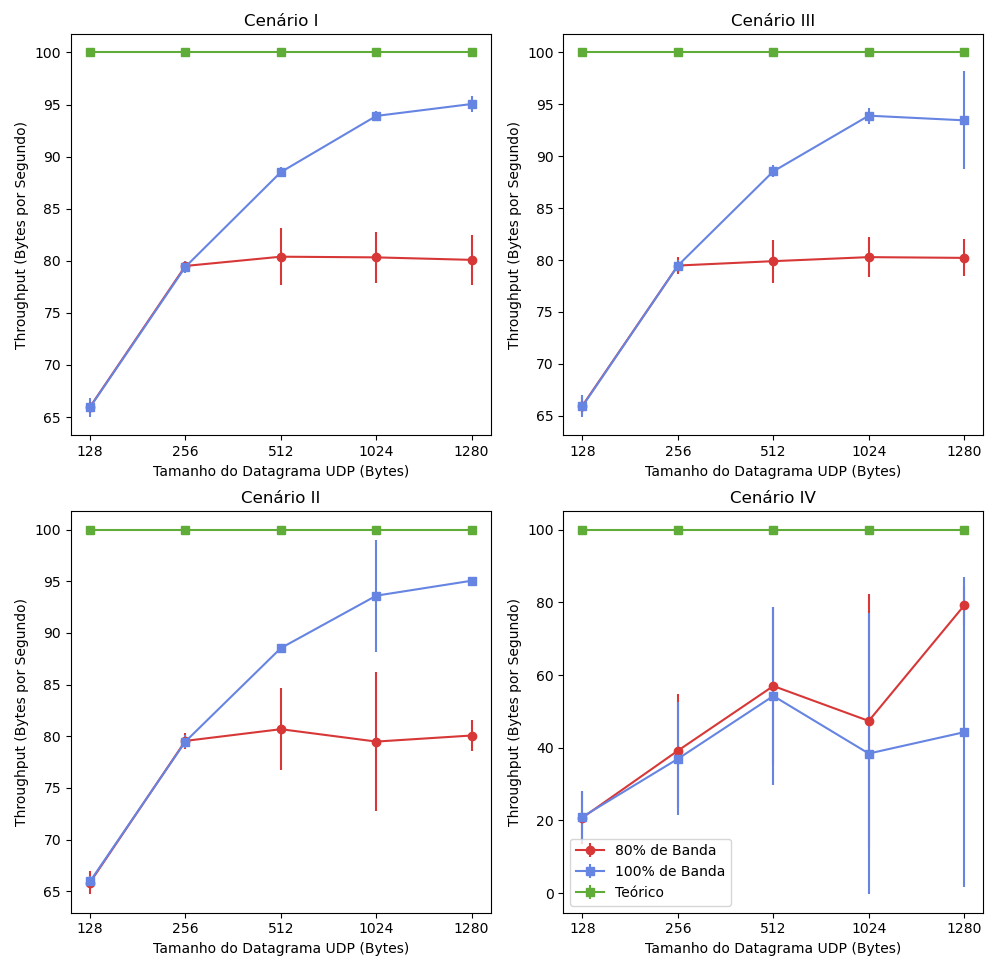
\includegraphics[width=0.9\linewidth]{sources/fig-throughput.png}
		\caption{\textit{Throughput} atingido com datagramas de tamanhos diferentes.}
    \label{fig:throughput}
\end{figure}

Como é possível notar na figura \ref{fig:throughput} o cenário de controle, isto é o I, possuio a maior taxa de transferência entre todos os cenários. Os cenários II e III tiveram resultados semelhantes porém, o II teve uma taxa ligeiramente superior nos datagramas maiores em comparação com o cenário III, isto é com uma variância maior também. Já o cenário IV teve o pior dos resultados registrados, com taxas de transferência inferior aos demais e com uma varianção elevada.

\subsubsection{Número de Pacotes}

\begin{figure}[H]
    \centering
    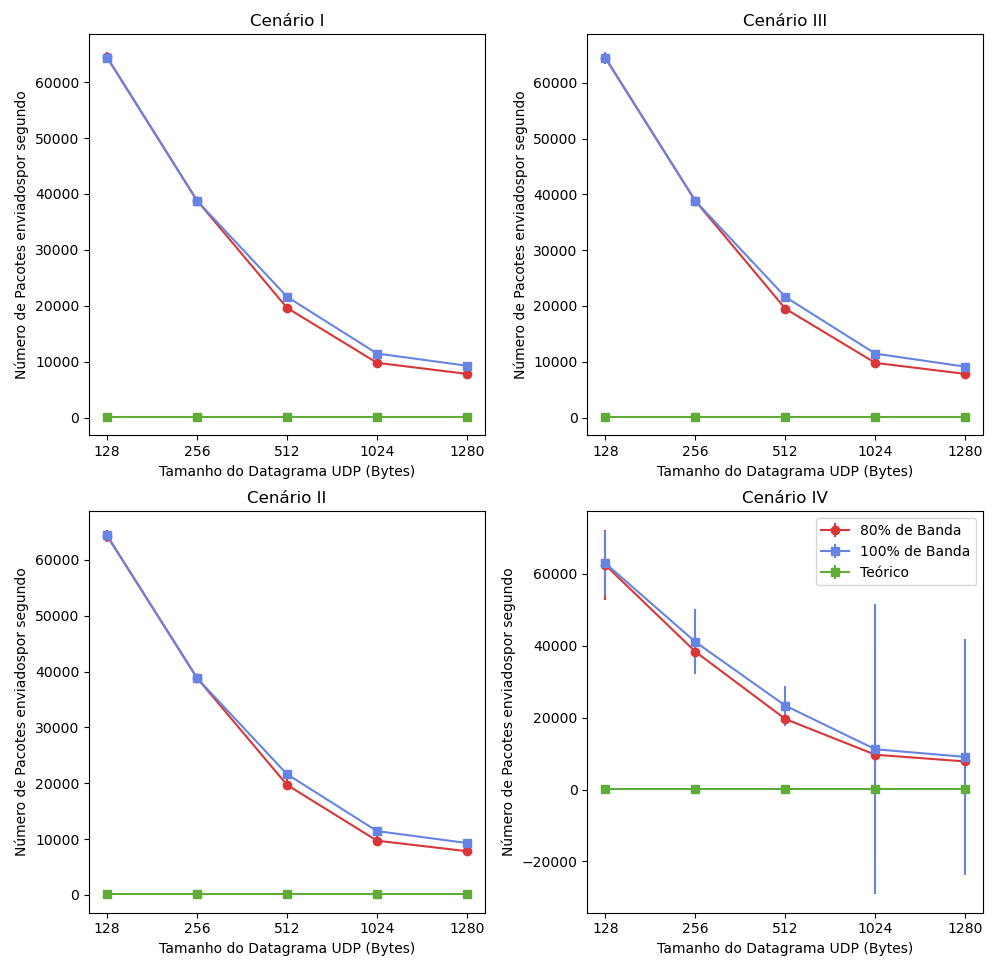
\includegraphics[width=0.9\linewidth]{sources/fig-pacotes.png}
    \caption{Número de datagramas enviados por segundo em cada teste realizado.}
    \label{fig:num pacotes}
\end{figure}

Assim como nos outro gráfico \ref{fig:throughput}, podemos notar um padrão. Ná figura \ref{fig:num pacotes} podemos notar pouca diferenca entre os cenários I, II e III, onde todos apresentam um número de pacotes enviados por segundo semelhante. É possível notar que novamente o cenário IV possuiu resultados bem diferentes dos demais, apresentando desvio padrão muito superior que os demais cenários, principalmente nos datagramas com tamanho de 1024 bytes.

\subsubsection{Jitter}

\begin{figure}[H]
    \centering
    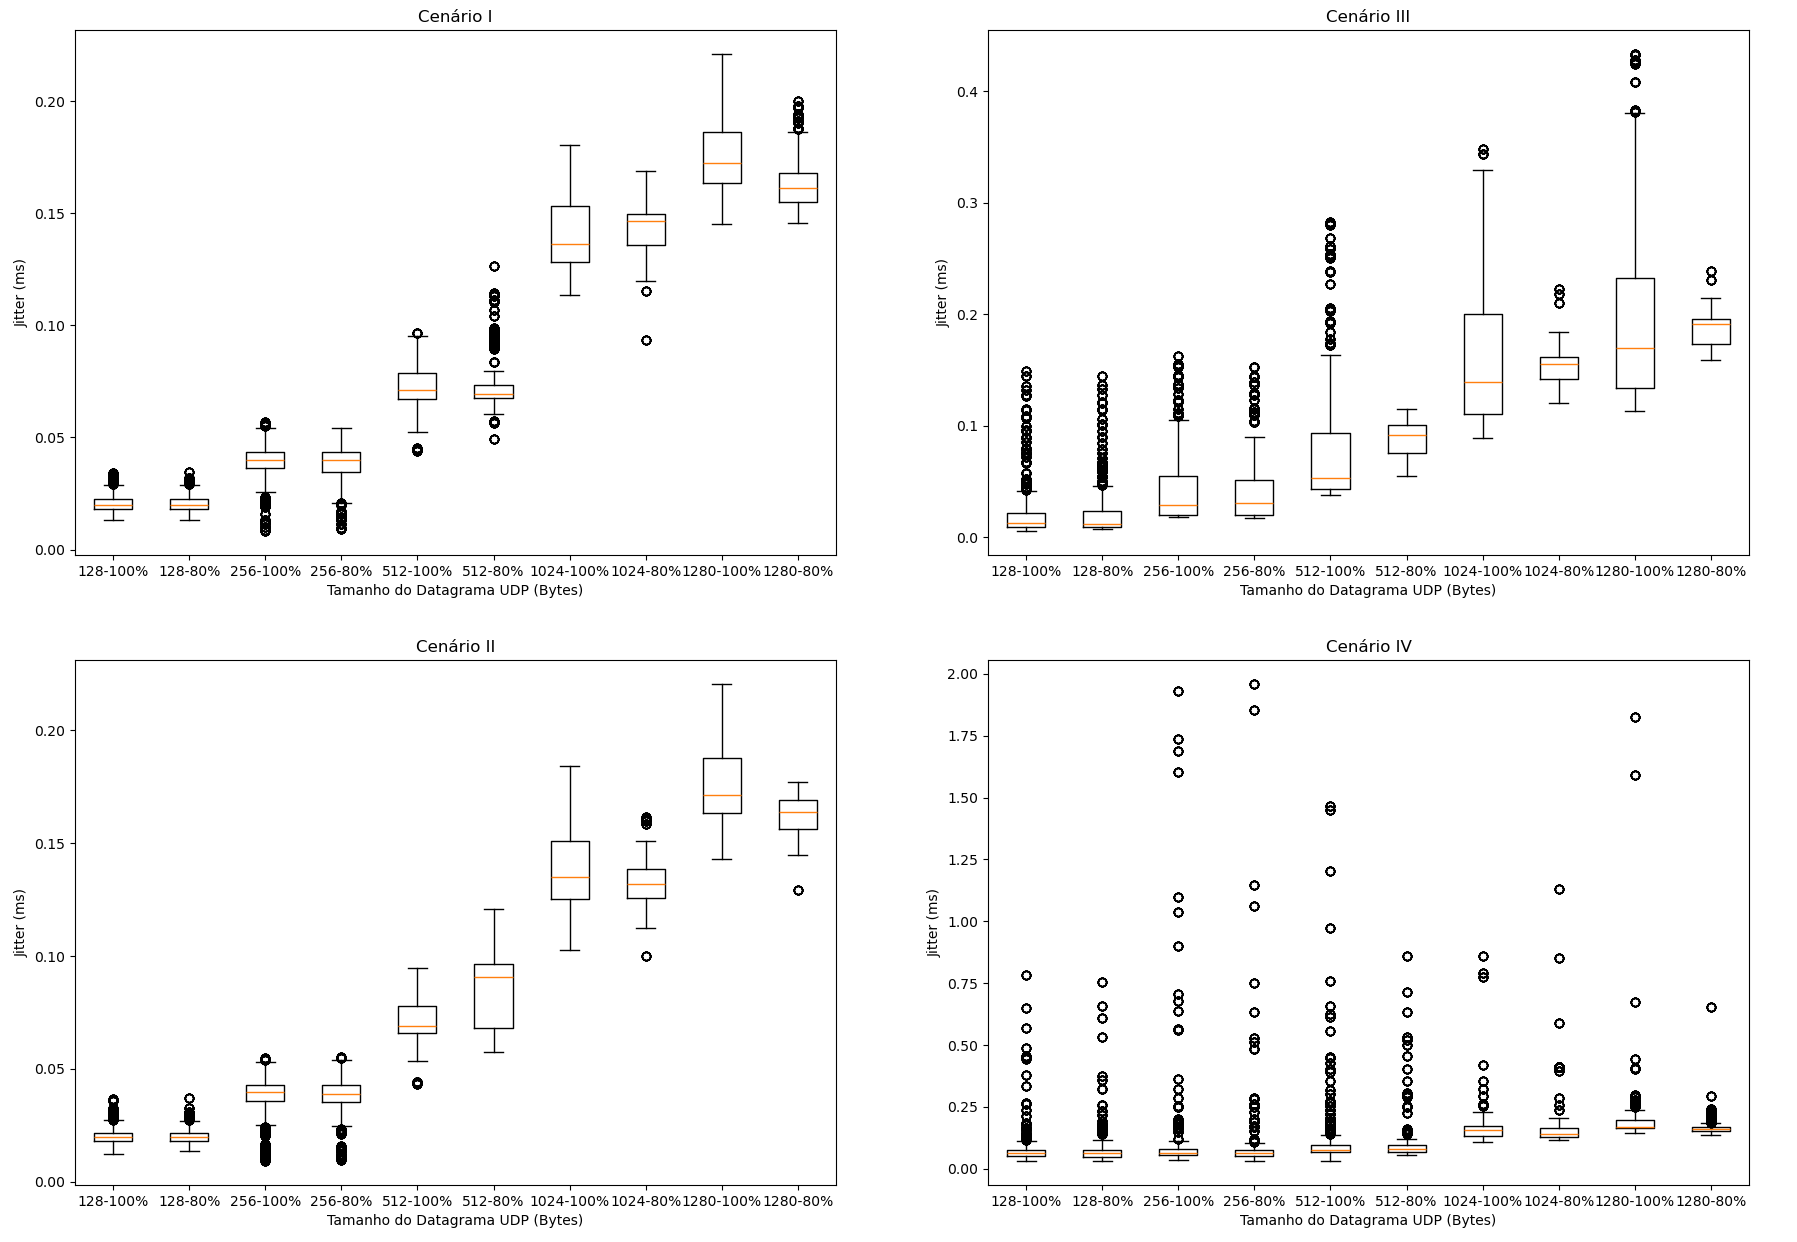
\includegraphics[width=0.9\linewidth]{sources/fig-jitter.png}
    \caption{Boxplot dos dados de jitter coletados nos testes seguindo tamanho de datagrama.}
    \label{fig:jitter}
\end{figure}

Nesta figura \ref{fig:jitter} podemos analizar as médias assim como os \textit{outliers} coletados pelo iPerf3 quando medindo o jitter. Como podemos notar o cenário I e II tiveram resultados semelhantes. O cenário III por sua vez teve um \textit{jitter} superior aos cenários I e II e com um \textit{outliers} mais notáveis. O cenário IV teve o pior dos resultados comparado com os demais, apresentando latências muito superiores e variações altissímas.

\subsubsection{Perda de Pacotes}

\begin{figure}[H]
    \centering
    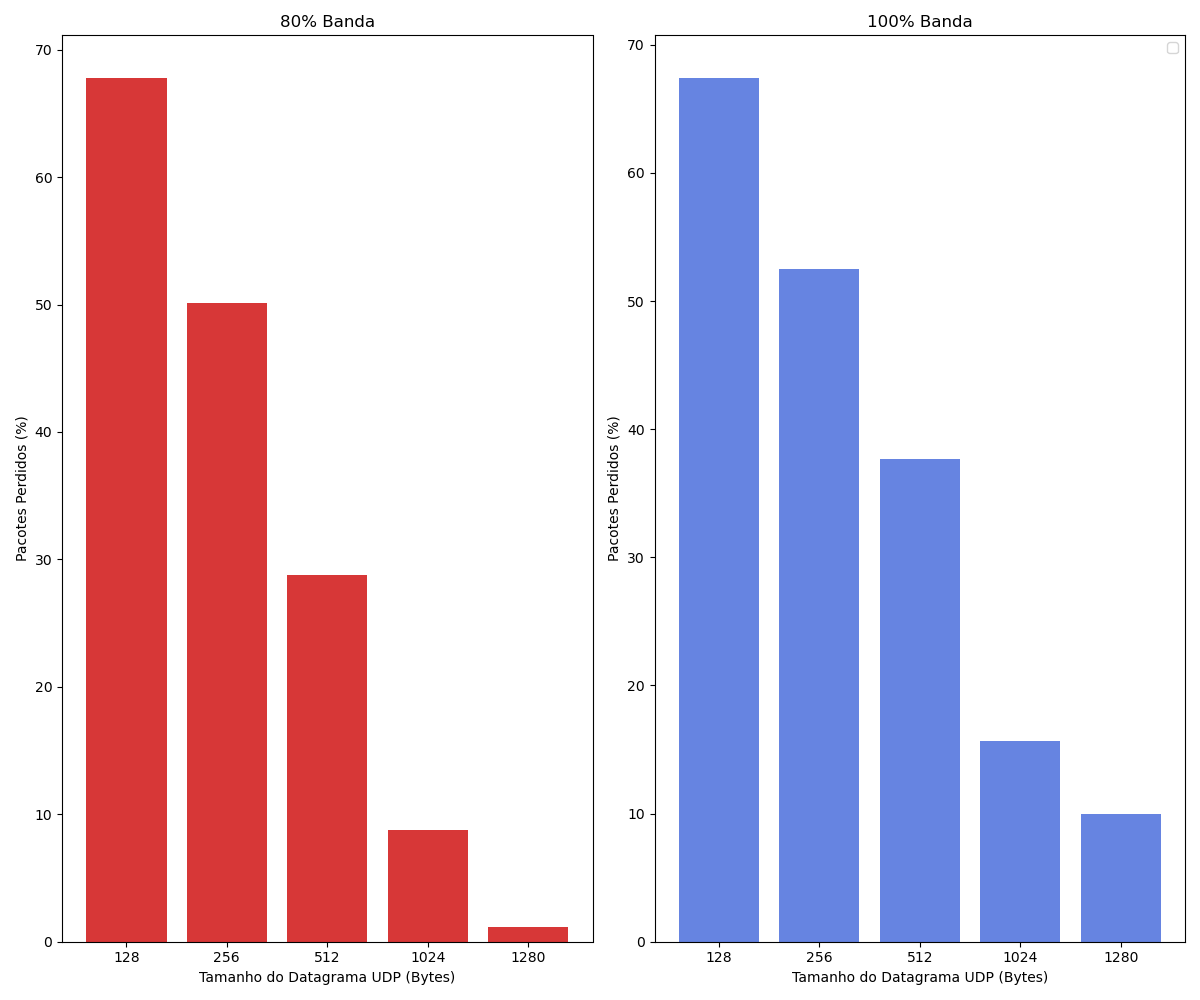
\includegraphics[width=0.9\linewidth]{sources/fig-pacotes-perdidos.png}
    \caption{Perda de Pacotes.}
    \label{fig:perda}
\end{figure}

Nesta figura \ref{fig:perda} é apenas exposto a perda de pacotes acosionada no cenário IV. Os demais cenários não apresentaram perdas de pacotes significativas, isto é, perdas superiores a 1\%. É claramente visível que o roteador deste cenário não foi capaz de suportar tal carga, tendo casos que as perdas ultrapassam 67\%. 

É possível notar que o roteador teve maior dificuldade lidando com datagramas menores, isso se dá porque o maior custo computacional acontece na quebra do cabeçalho. Então em fluxos com datagramas menores mais pacotes são enviados e por consequencia mais pacotes precisam ser desmontados pelo roteador. Já com datagramas maiores o número de pacotes pode ser menor como é visto na figura\ref{fig:num pacotes}.






